\newpage
\section{Versuchsaufbau}
\label{sec:Aufbau}

Die Gamma-Strahlung einer \ce{^{137}Cs}
Quelle wird durch eine Blende kollimiert und trifft auf eine Probe in Form
eines Würfels.
In Strahlrichtung hinter dem Würfel befindet sich ein NaJ-Detektor.
Von diesem Szitillationsdetektor werden Pulse erzeugt
und nach einer Verstärkung in einen Multichannelanalyser gegeben.
Dieser ist an einen Computer angeschlossen,
auf welchem mittels des Programms \texttt{MAESTRO}
das erstellte Histogramm ausgelesen und gespeichert wird.
Der Versuchsaufbau befindet sich mit Ausnahme des Computers hinter einem
Schutz aus Bleiklötzen, um eine Strahlungsaufnahme möglichst zu vermeiden.
Als Proben werden vier Würfel verwendet.
Der Erste besteht ausschließlich aus einem Aluminiumgehäuse, der Zweite und Dritte
bestehen aus zu bestimmenden Stoffen in einem Aluminiumgehäuse
und der Vierte Würfel beherbergt in dem Aluminiumgehäuse $3 \times 3 \times 3$
kleine Würfel.
Jeder Würfel wird vertikal so positioniert, dass die mittlere Ebene analysiert
werden kann. Weiterhin ist der Probenhalter horizontal verschieb- und drehbar.

\section{Durchführung}
\label{sec:Durchführung}

Im Programm \texttt{MAESTRO} werden für jede Messung die Marker so positionert,
dass nur der Photopeak des Sprektrums vermessen wird.
Nach dem Aufnehmen eines Spektrums
wird mit einem Rechtsklick auf den markierten Bereich und auf
\texttt{MCB Properties} das Maximum des markierten Bereichs angezeigt.
Zu Beginn wird die Messzeit auf \SI{60}{\second} eingestellt und das Spektrum
der verwendeten Quelle ohne Probe vermessen. Im Anschluss werden die
Würfel \num{1} und \num{2} eingesetzt und bei einer Messzeit von
\SI{60}{\second} für Würfel \num{1} und \SI{480}{\second} für Würfel \num{2}
aus jeweils vier verschiedenen Positionen vermessen. Die Positionen sind
in Abbildung \ref{fig:wuerfelpos} als
$I_{1}, I_{2}, I_{11}$ und $I_{12}$ eingezeichnet.
Die Messzeit ist so zu wählen, dass die statistische Unsicherheit kleiner
als \SI{3}{\percent} ist, also im Photopeak mindestens circa \num{1112}
Ereignisse registriert werden.
Zuletzt wird Würfel vier eingesetzt und alle \num{12} in Abbildung
\ref{fig:wuerfelpos} dargestellten Strahlengänge vermessen. Dabei wird die
Messzeit auf \SI{480}{\second} eingestellt.

\begin{figure}
  \centering
  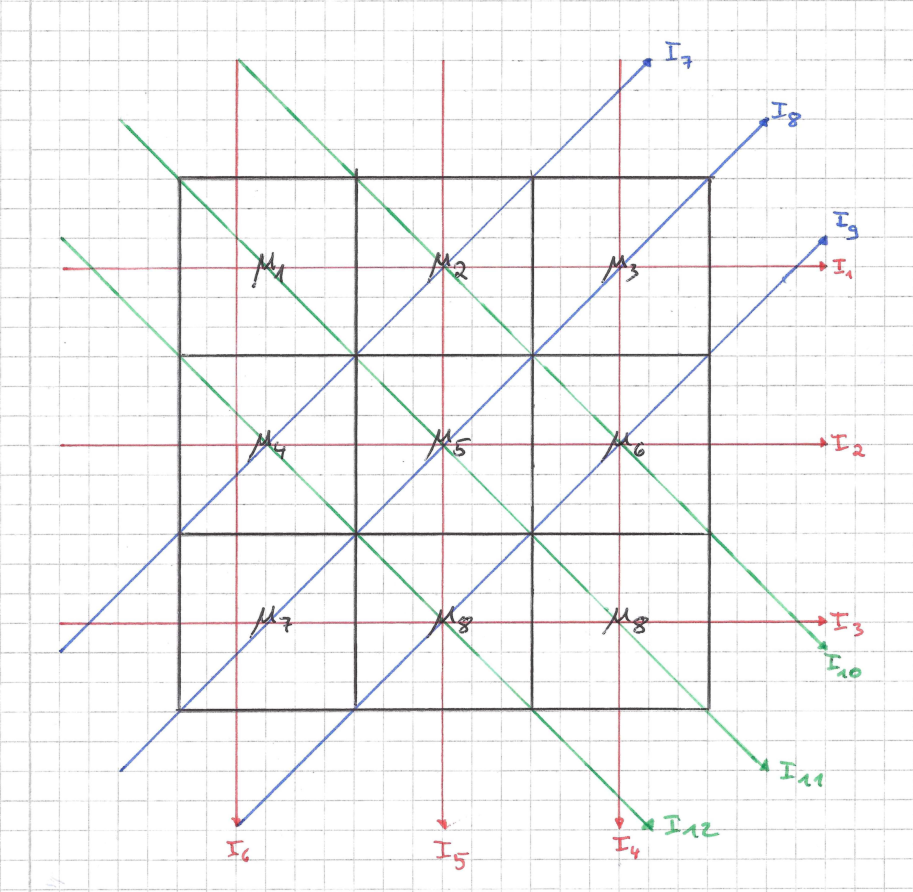
\includegraphics[height=8.0cm]{content/wuerfelpos.pdf} % height=8.0cm
  \caption{Die verschiedenen Strahlengänge durch die Würfelprobe.}
  \label{fig:wuerfelpos}
\end{figure}
